
\documentclass{report}

\usepackage[utf8]{inputenc}
\usepackage[italian]{babel}
\usepackage{import}
\usepackage{todonotes}
\usepackage{color}
\usepackage{rotating}
\usepackage[hidelinks]{hyperref}
\usepackage{url}
\usepackage{pdfpages}
\usepackage{siunitx}
\usepackage{pdflscape}
\usepackage{subfig}
\usepackage[euler]{textgreek}
\usepackage{mhchem}

\usepackage{multirow}

\usepackage{enumerate} 
\usepackage{amsmath}
\usepackage{amsfonts}

\usepackage[signatures,swapnames,sans]{frontespizio}

\usepackage{geometry}
\geometry{portrait, margin=3cm}
\usepackage{siunitx}
\usepackage{booktabs}

\renewcommand*\figurename{Figura}

\newcommand{\sub}[1]{\textsubscript{#1}}
\newcommand{\super}[1]{\textsuperscript{#1}}
\newcommand{\parallelsum}{\mathbin{\!/\mkern-5mu/\!}}

\newcommand{\Fig}[0]{Fig.}

\usepackage{titlesec}

\titleformat{\chapter}{\normalfont\huge}{}{20pt}{\huge\bfseries}

\linespread{1.3}


%% COMANDI UTILI
%\begin{table}[h]
%	\centering
%	\begin{tabular}{|c|c|c|}
%	\cline{2-3} 
%	\multicolumn{1}{c|}{} & \textbf{Valore nominale} & \textbf{Valore misurato}\\ 
%		%\hline
%		%{} & \textbf{Valore nominale} & \textbf{Valore misurato} \\ 
%		\hline
%		$\mathbf{R_1}$ & \SI{18}{k\ohm} & \SI{17.977}{k\ohm} \\ 
%		\hline
%		$\mathbf{R_2}$& \SI{1.8}{k\ohm} & \SI{1.815}{k\ohm} \\ 
%		\hline
%	\end{tabular}
%\caption{Misure delle resistenze utilizzate per il circuito.}
%\label{table:mis_res}
%\end{table}
%\begin{figure}[h!]
%\centering
%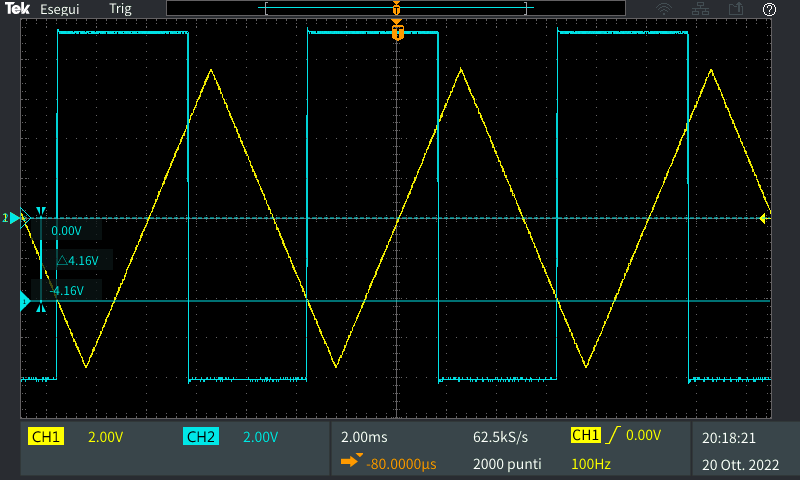
\includegraphics[height=6.5cm]{immagini/TEK00018}\\(a)\\[1ex]
%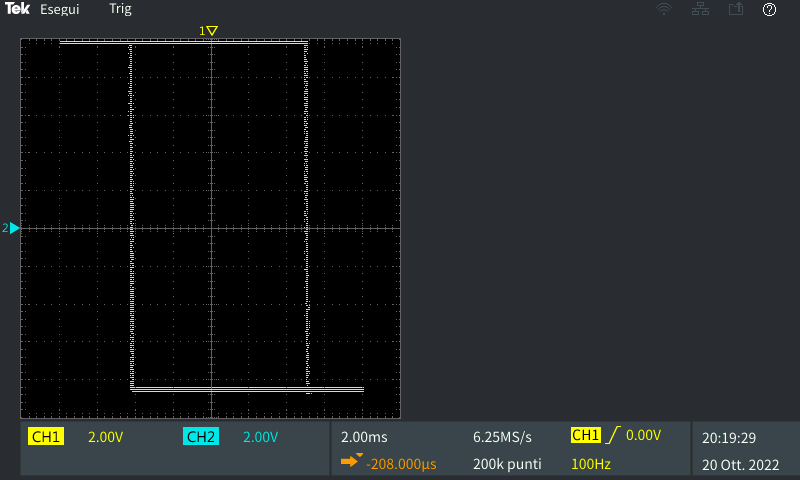
\includegraphics[height=6.5cm]{immagini/TEK00019}\\(b)
%\caption{Risposta del circuito con accoppiamento DC (a) e accoppiamento AC (b).}
%	\label{figura:accopp}
%\end{figure}

\begin{document}
\addtocounter{chapter}{+2}
	\begin{frontespizio}
		\Margini{3cm}{3cm}{3cm}{3cm}
		\Universita{Bergamo}
		\Logo[43.332mm]{unibg-mark}
		\Divisione{Scuola di Ingegneria}
		\Corso[Laurea Magistrale]{Ingegneria Informatica}
		\Titolo{Laboratorio di Elettronica}
		\Sottotitolo{Relazione esperienza di laboratorio 3}
		\Punteggiatura{}
		\NRelatore{Prof.}{Prof.}
		\Relatore{Luigi Gaioni}
		\Candidato[1058231]{Giulia Allievi}
		\Candidato[1059640]{Martina Fanton}
		\Annoaccademico{2022--2023}
		\begin{Preambolo*}
			\usepackage[italian]{babel}
			\usepackage[T1]{fontenc}
			\usepackage[utf8]{inputenc}
			\usepackage{microtype}
			\usepackage{lmodern}
			\graphicspath{{img/}}
			
			\renewcommand{\frontinstitutionfont}{\fontsize{14}{17}\bfseries\scshape}
			\renewcommand{\fronttitlefont}{\fontsize{17}{21}\bfseries\scshape}
			\renewcommand{\frontfootfont}{\fontsize{12}{14}\bfseries\scshape}
		\end{Preambolo*}
	\end{frontespizio}

%----------------------------------------------------------------------------------------
%	PAGINA BIANCA
%----------------------------------------------------------------------------------------
\newpage
\null
\thispagestyle{empty}
\newpage

%----------------------------------------------------------------------------------------
%	INTRO
%----------------------------------------------------------------------------------------
\chapter{Relazione attività di laboratorio 3}
%\section*{Introduzione}
%In questo laboratorio, sono stati analizzati circuiti composti da diodi e/o da amplificatori operazionali.
%In particolare il primo circuito analizzato permette di risolvere un problema che si verificava nell'ultimo circuito analizzato durante il precedente laboratorio, ovvero nel raddrizzatore a doppia semionda. Questo problema consisteva nella presenza di una differenza di tensione, idealmente pari a \SI{0.7}{\volt} (mentre nelle nostre misure risultava pari a \SI{0.460}{\volt}), tra il segnale in uscita e quello in ingresso.
%\\Il secondo circuito invece è un trigger di  Schmitt, che presenta nella sua caratteristica tra la tensione di ingresso e quella di uscita un ciclo di isteresi.
%\\Infine il terzo circuito e il quarto funzionano senza la necessità di applicare un segnale in ingresso.
%% DA SISTEMARE

%\newpage
\section{Circuito 1: raddrizzatore a doppia semionda di precisione}
\subsection{Schema del circuito e Funzione di Trasferimento}
Questo circuito, come si può notare dalla figura \ref{figura:schema1}, presenta due amplificatori operazionali, di cui quello in alto è retroazionato negativamente, e un diodo.
\begin{figure}[h]
	\centering
	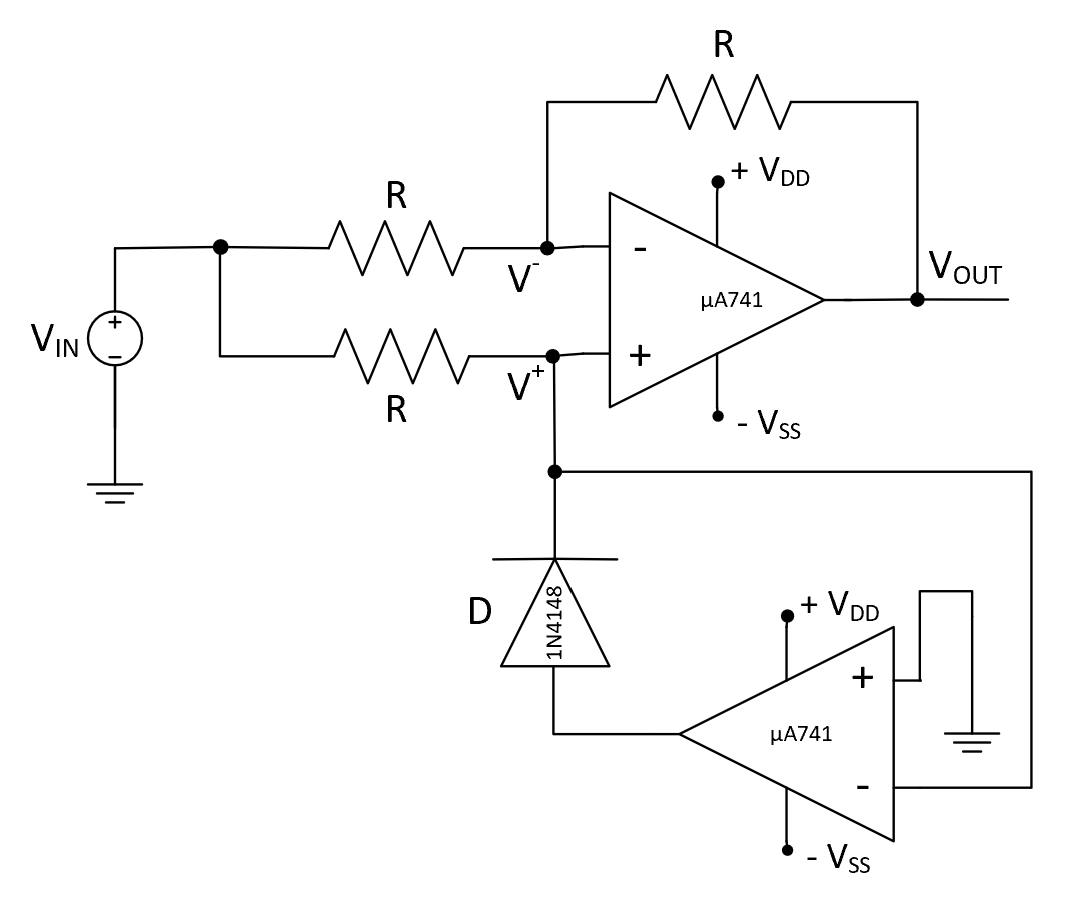
\includegraphics[height=7.5cm]{immagini/schema1}
	\caption{Schema del raddrizzatore a doppia semionda di precisione.}
	\label{figura:schema1}
\end{figure}
\\ \noindent La funzione di trasferimento di questo raddrizzatore è:
\begin{equation}
   \begin{cases}
   V_{in}< \SI{0}{\volt}\;\;\indent\indent\rightarrow \mathrm{D\;ON}\;\;\;\; \Rightarrow V_{out} = -V_{in}\\
   V_{in}\ge \SI{0}{\volt}\;\;\indent\indent\rightarrow \mathrm{D\; OFF}\;\; \Rightarrow V_{out} = V_{in}
   \end{cases}
\end{equation}
Da questa funzione di trasferimento si può notare che l'uscita non risulta shiftata rispetto all'ingresso, come invece succedeva nel raddrizzatore a doppia semionda analizzato durante lo scorso laboratorio. Dunque questo circuito permette di risolvere il problema della differenza di tensione presente tra uscita e ingresso. Di conseguenza, in uscita si ottiene un segnale analogo a quello in ingresso, ma in cui le semionde risultano raddrizzate.
\subsection{Analisi e dati sperimentali}
Per la realizzazione del circuito sulla breadboard (visibile nella figura \ref{figura:circuito1}) abbiamo deciso di utilizzare due amplificatori operazionali di tipo \textmu A741, che sono amplificatori operazionali \textit{general purpose}, e un diodo di tipo 1N4148.
Invece per quanto riguarda i valori delle resistenze abbiamo utilizzato resistenze da \SI{12}{k\ohm}, le cui misure sono state riportate nella tabella \ref{table:mis_res1}.
\begin{table}[h!]
	\centering
	\begin{tabular}{|c|c|c|}
		\cline{2-3} 
		\multicolumn{1}{c|}{} & \textbf{Valore nominale} & \textbf{Valore misurato}\\ 
		\hline
		$\mathbf{R_1}$ & \SI{12}{k\ohm} & \SI{11.802}{k\ohm} \\ 
		\hline
		$\mathbf{R_2}$ & \SI{12}{k\ohm} & \SI{11.947}{k\ohm} \\ 
		\hline
		$\mathbf{R_3}$ & \SI{12}{k\ohm} & \SI{11.885}{k\ohm} \\ 
		\hline
	\end{tabular}
	\caption{Misure delle resistenze utilizzate per il circuito.}
	\label{table:mis_res1}
\end{table}
\begin{figure}[h]
	\centering
	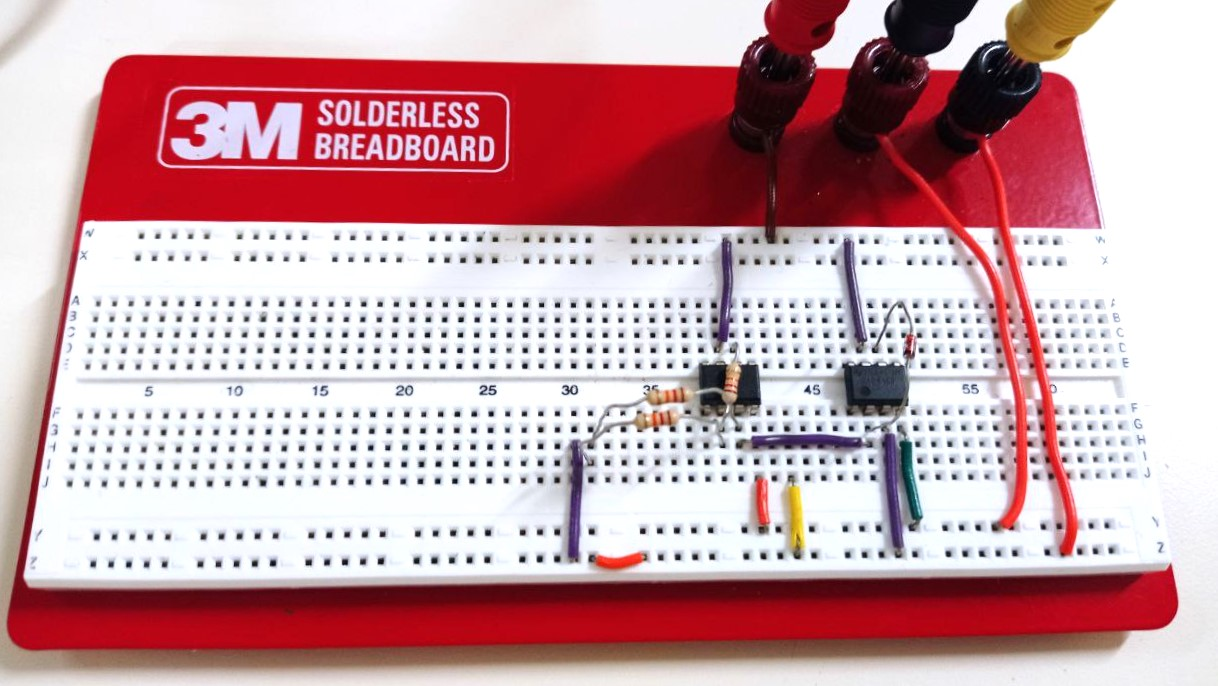
\includegraphics[height=6.5cm]{immagini/circuito1}
	\caption{Fotografia del raddrizzatore a doppia semionda di precisione realizzato in laboratorio.}
	\label{figura:circuito1}
\end{figure}
\\\indent Dopo aver realizzato il circuito sulla breadboard, sono state collegate sia le alimentazioni (con un valore di \SI{+10}{\volt} per l'alimentazione positiva e di \SI{-10}{\volt} per quella negativa) sia il segnale d'ingresso, con un'ampiezza picco-picco di \SI{2}{\volt} e frequenza prima di  \SI{100}{\hertz},  e poi pari a \SI{1}{k\hertz}.\par
Il segnale in uscita prodotto dall'oscilloscopio lo si può vedere nella figura \ref{figura:uscita11}. Per queste due frequenze sono state analizzate anche le rappresentazioni XY, ovvero la caratteristica tra tensione di ingresso e tensione di uscita del circuito (in figura \ref{figura:xyuscita1}).
\begin{figure}[h!]
	\centering
	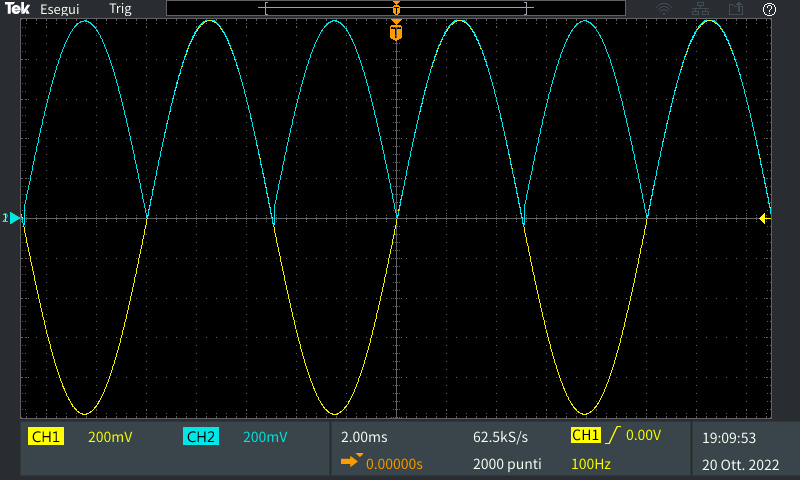
\includegraphics[height=4.6cm]{immagini/TEK00000}
	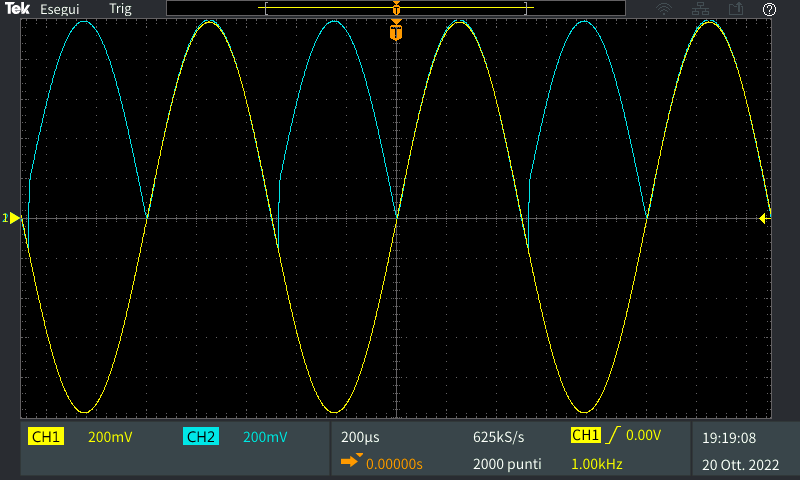
\includegraphics[height=4.6cm]{immagini/TEK00003}
	\caption{Risposta del circuito con $\mathrm{f= \SI{100}{\hertz}}$ (sinistra) e con $\mathrm{f= \SI{1}{k\hertz}}$ (destra).}
	\label{figura:uscita11}
\end{figure}
\begin{figure}[h!]
	\centering
	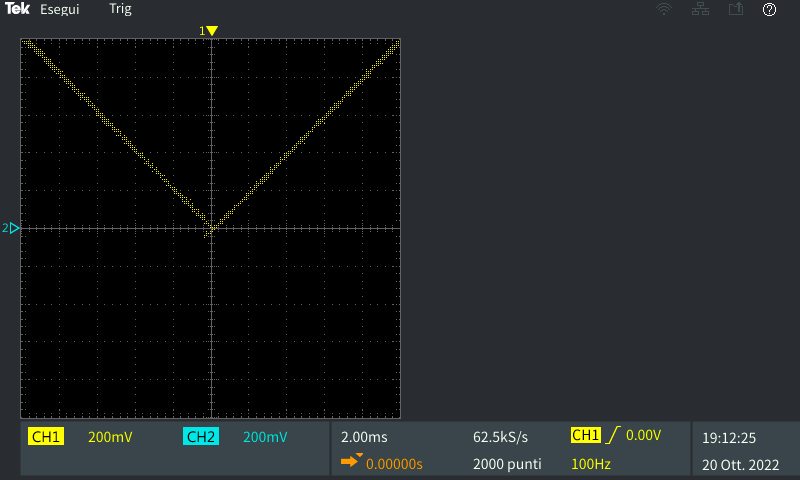
\includegraphics[height=4.6cm]{immagini/TEK00001}
	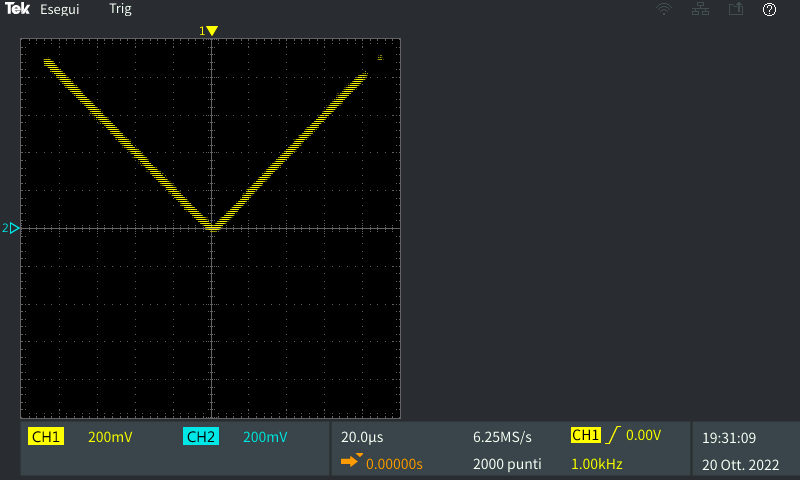
\includegraphics[height=4.6cm]{immagini/TEK00010}
	\caption{Rappresentazione XY della risposta del circuito con $\mathrm{f= \SI{100}{\hertz}}$ (sinistra) e con $\mathrm{f= \SI{1}{k\hertz}}$ (destra).}
	\label{figura:xyuscita1}
\end{figure}
\\In tutti questi grafici il segnale presenta un andamento quasi ideale, ma nella parte iniziale delle semionde negative raddrizzate si possono notare dei tratti anomali vicino all'asse delle ascisse. Nel grafico XY, lo vediamo perché il segnale non si trova solo nel primo e nel secondo quadrante, ma c'è un tratto (seppur molto breve) anche nel terzo quadrante. Queste anomalie sono dovute al fatto che \todo{quando il segnale in ingresso è positivo, il diodo è spento, quindi il secondo OPAMP (quello in basso) lavora in anello aperto. La sua tensione in uscita è pari a $\displaystyle\mathrm{V_{SS}}$, come si vede in figura \ref{figura:uscita111}, perciò impiegherà un certo tempo per erogare una tensione positiva, di conseguenza il diodo non si accende istantaneamente}{l'OPAMP in basso può avere una retroazione aperta per la presenza del diodo e quindi la sua uscita deve svolgere uno swing abbastanza ampio (visualizzato nella figura \ref{figura:uscita111}) per far arrivare la sua uscita al valore dell'alimentazione.} Questo poi incide anche sulla velocità del sistema nel raddrizzare il primo tratto delle semionde negative.
\begin{figure}[h!]
	\centering
	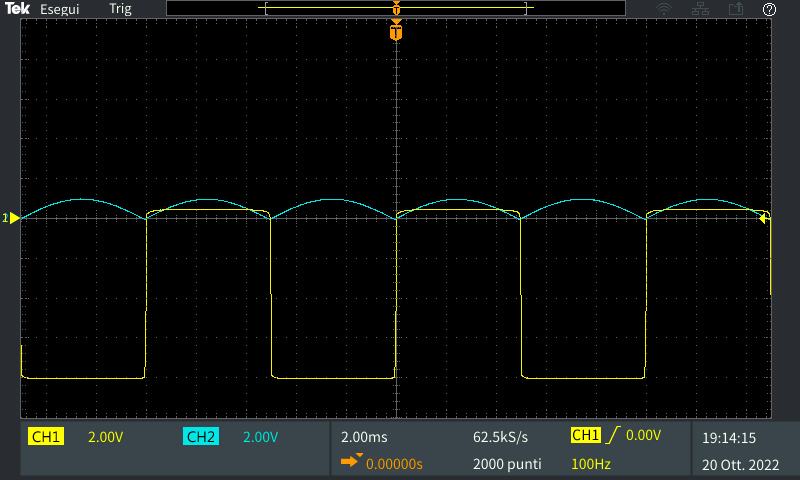
\includegraphics[height=4.6cm]{immagini/TEK00002}
	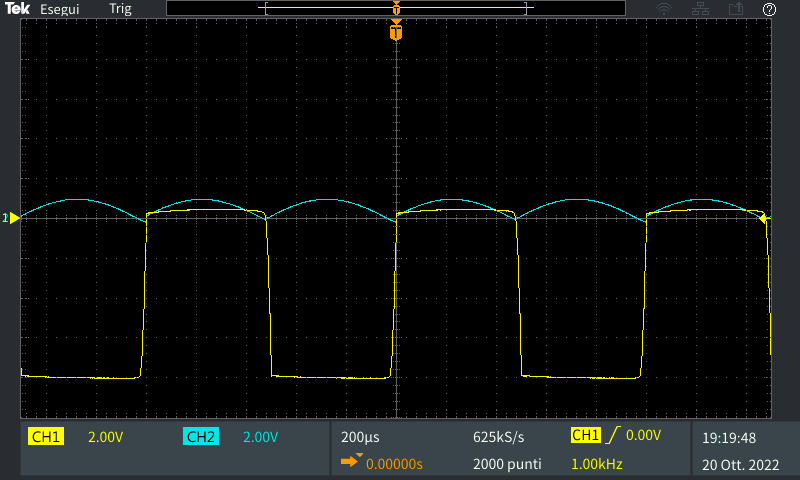
\includegraphics[height=4.6cm]{immagini/TEK00004}
	\caption{Risposta dell'OPAMP in basso con $\mathrm{f= \SI{100}{\hertz}}$ (sinistra) e con $\mathrm{f= \SI{1}{k\hertz}}$ (destra).}
	\label{figura:uscita111}
\end{figure}
\\Analizzando invece frequenze maggiori (ad esempio \SI{10}{k\hertz}), il segnale presenta delle anomalie di maggiore rilevanza rispetto alle precedenti, come si può notare nella figura \ref{figura:uscita12}. Le semionde positive sono poco distorte, infatti vengono solo leggermente ritardate, invece sulle semionde negative si vede chiaramente l'escursione di tensione provocata dall'operazionale che si trova in anello aperto. Queste anomalie derivano dal fatto che l'OPAMP non è adatto a operare in alta frequenza quando presenta un anello che può risultare aperto.
\begin{figure}[h!]
	\centering
	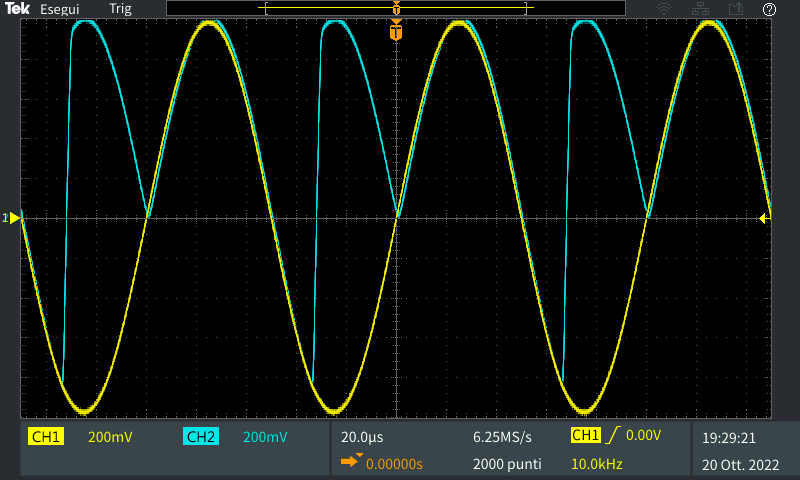
\includegraphics[height=6.5cm]{immagini/TEK00008}
	\caption{Risposta del circuito con $\mathrm{f= \SI{10}{k\hertz}}$.}
	\label{figura:uscita12}
\end{figure}
\newpage
\section{Circuito 2: trigger di Schmitt}
\subsection{Schema del circuito e Funzione di Trasferimento}
In questo circuito è presente un amplificatore operazionale non retroazionato negativamente, ma con una retroazione positiva, quindi il circuito opera come un comparatore.\par
La rete di reazione positiva è formata da un partitore resistivo, in cui inizialmente utilizzeremo due resistenze dello stesso valore per analizzare la risposta del circuito in maniera più semplice, come si può vedere dallo schema di figura \ref{figura:schema2}.\par
La particolarità del trigger di Schmitt è che, a differenza dei normali comparatori, la caratteristica ingresso-uscita presenta un'isteresi, di conseguenza questo circuito è immune a eventuali disturbi presenti in ingresso. In un comparatore semplice infatti, se il segnale in ingresso è rumoroso su valori prossimi alla soglia ${V^+}$, si possono avere delle transizioni involontarie dell'uscita da ${V_{DD}}$ a ${V_{SS}}$, perciò il rumore in ingresso rende anche l'uscita rumorosa. Questo problema viene risolto nel trigger di Schmitt, perché una volta attraversata una soglia (per esempio ${V_H^+}$ ) quest'ultima varierà il suo valore e si sposterà sul secondo valore (${V_L^+}$), quindi l'uscita non cambia finché non si attraversa la seconda soglia, rendendo il circuito robusto rispetto ai rumori presenti sulle linee d'ingresso.\par
\begin{figure}[h]
	\centering
	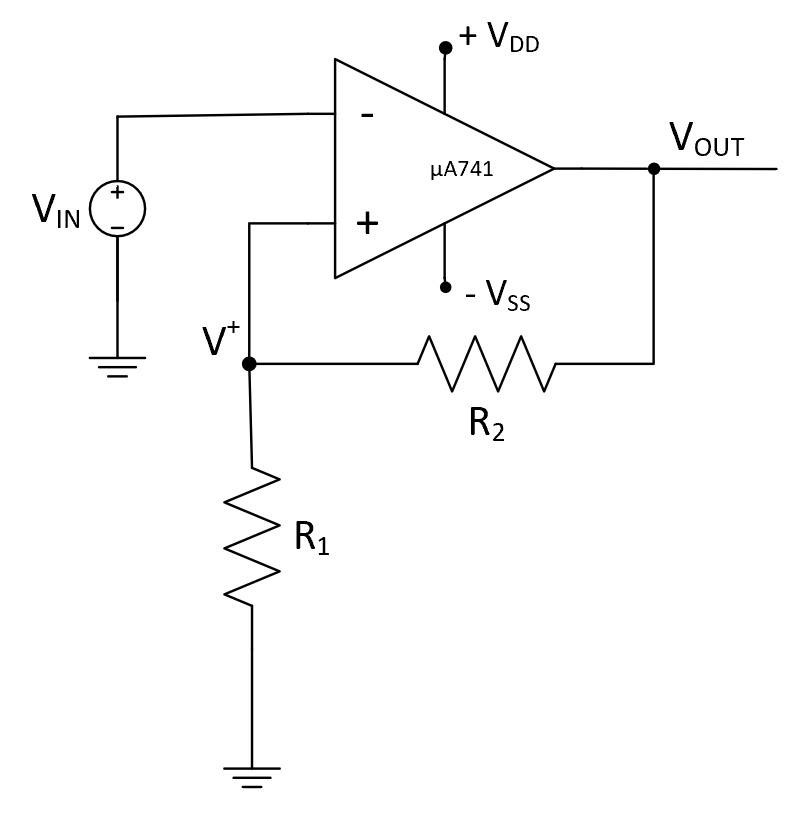
\includegraphics[height=7.5cm]{immagini/schema2}
	\caption{Schema del trigger di Schmitt.}
	\label{figura:schema2}
\end{figure}
La funzione di trasferimento di questo comparatore è:\\
\begin{equation}
   \begin{cases} % da controllare
   V_{out}= V_{DD}\;\indent\indent \mathrm{per\;}  V_L^+<V_{in}<V_H^+\mathrm{, \;\; con\;}\displaystyle{ V_H^+=\frac{R_1}{R_1+R_2}\cdot V_{DD}=\frac{V_{DD}}{2}}\mathrm{\;\;\;\; se \;} R_1=R_2\\[10pt]
   V_{out}= V_{SS}\;\;\indent\indent \mathrm{per\;} V_H^+<V_{in}<V_L^+\mathrm{, \;\; con\;}\displaystyle{ V_H^+=\frac{R_1}{R_1+R_2}\cdot |V_{SS}|=\frac{|V_{SS}|}{2}}\mathrm{\;\; se \;} R_1=R_2\\
   \end{cases}
\end{equation}
% SISTEMARE FDT
%\begin{equation}
%	\begin{cases} % da controllare
%		V_{out}= V_{DD}\;\indent\indent \mathrm{per\; t\; da\;} V_{in}=V_L^+\mathrm{\; a\;}V_{in}=V_H^+\mathrm{, \;\; con\;}\displaystyle{ V_H^+=\frac{R_1}{R_1+R_2}\cdot V_{DD}=\frac{V_{DD}}{2}}\mathrm{\;\;\;\; se \;} R_1=R_2\\[10pt]
%		V_{out}= V_{SS}\;\;\indent\indent \mathrm{per\; t\; da\;} V_{in}=V_H^+\mathrm{\; a\;}V_{in}=V_L^+\mathrm{, \;\; con\;}\displaystyle{ V_H^+=\frac{R_1}{R_1+R_2}\cdot |V_{SS}|=\frac{|V_{SS}|}{2}}\mathrm{\;\; se \;} R_1=R_2\\
%	\end{cases}
%\end{equation}
\subsection{Analisi e dati sperimentali}
Per la realizzazione del circuito sulla breadboard (visibile nella figura \ref{figura:circuito2}) è stato utilizzato un amplificatore operazionale di tipo \textmu A741.
Invece per quanto riguarda i valori delle resistenze abbiamo utilizzato due resistenze da \SI{12}{k\ohm}, le cui misure sono state riportate nella tabella \ref{table:mis_res2}.
\begin{table}[h!]
	\centering
	\begin{tabular}{|c|c|c|}
		\cline{2-3} 
		\multicolumn{1}{c|}{} & \textbf{Valore nominale} & \textbf{Valore misurato}\\ 
		\hline
		$\mathbf{R_1}$ & \SI{12}{k\ohm} & \SI{11.802}{k\ohm} \\ 
		\hline
		$\mathbf{R_2}$ & \SI{12}{k\ohm} & \SI{11.947}{k\ohm} \\ 
		\hline
	\end{tabular}
	\caption{Misure delle resistenze utilizzate per il circuito.}
	\label{table:mis_res2}
\end{table}
\begin{figure}[h]
	\centering
	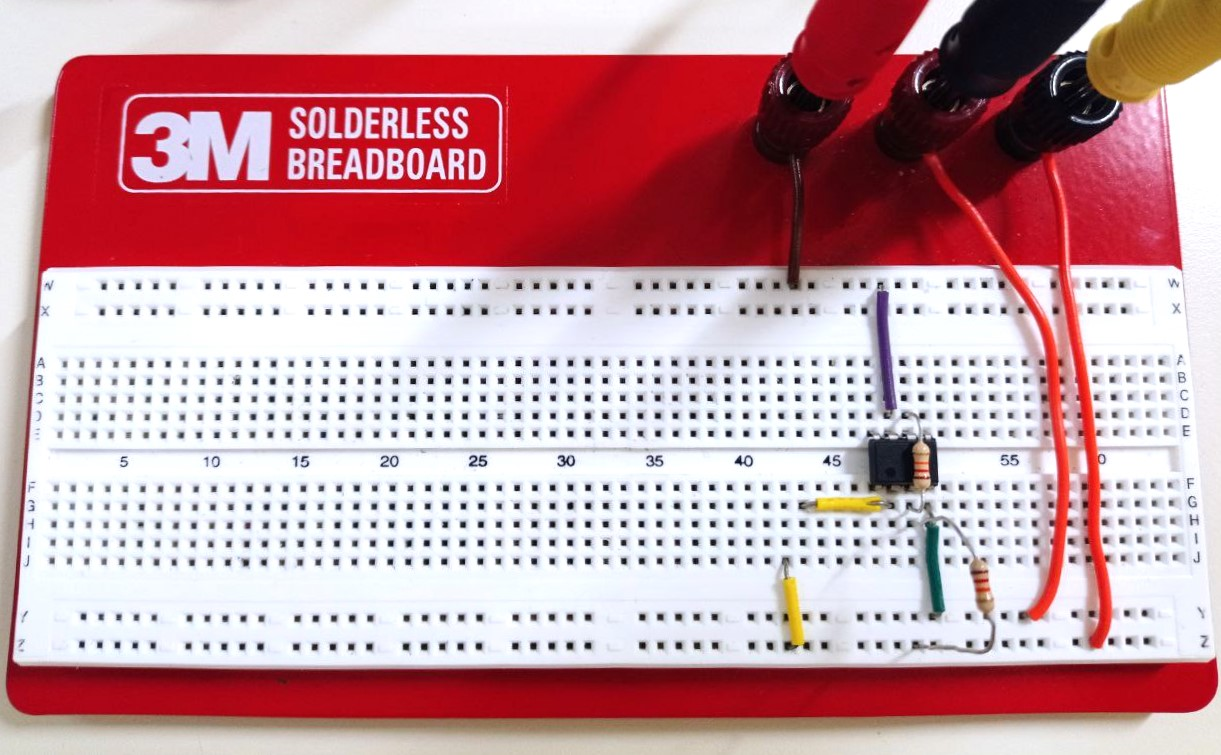
\includegraphics[height=7.5cm]{immagini/circuito2}
	\caption{Fotografia del trigger di Schmitt realizzato in laboratorio.}
	\label{figura:circuito2}
\end{figure}
\\Dopo aver realizzato il circuito sulla breadboard, scegliamo di applicare in ingresso un'onda triangolare con ampiezza picco-picco di \SI{15}{\volt}. Questo valore deve essere scelto in modo tale da poter vedere le transizioni da una soglia all'altra.\par
Per prima cosa abbiamo analizzato l'uscita del circuito con un segnale in ingresso con frequenza di \SI{100}{\hertz} (figura \ref{figura:uscita21}), dai grafici si può notare che il comportamento dei segnali risulta corretto. Abbiamo quindi misurate le due soglie, i cui valori sono risultati pari a \SI{4.88}{\volt} per ${V_H^+}$ (soglia positiva) e \SI{-4.16}{\volt} per ${V_L^+}$ (soglia negativa). Anche questi valori sono corretti, infatti corrispondono a circa metà della tensione che l'OPAMP eroga in uscita quando satura al valore positivo o negativo.
\begin{figure}[h!]
	\centering
	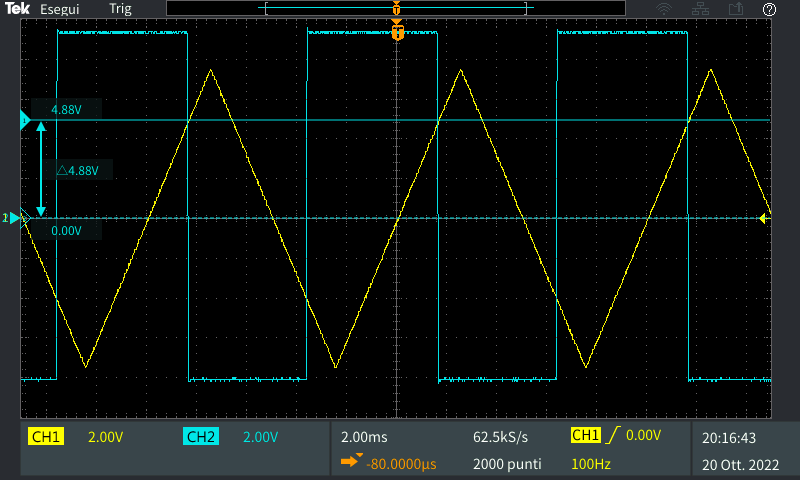
\includegraphics[height=4.6cm]{immagini/TEK00017}
	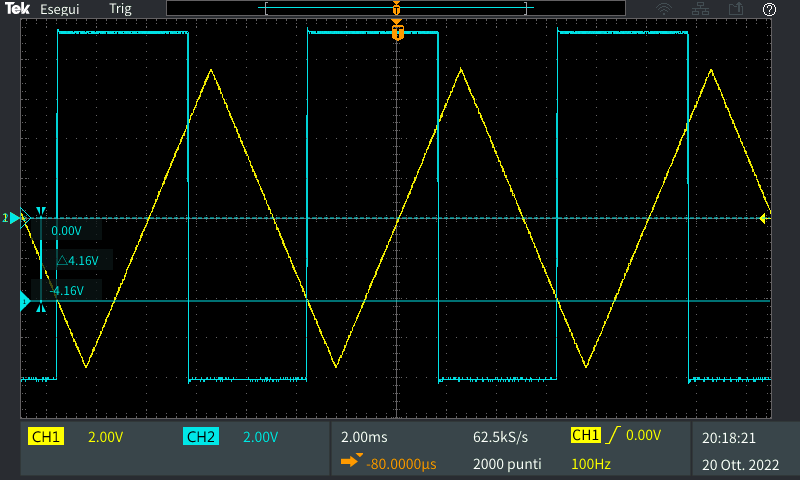
\includegraphics[height=4.6cm]{immagini/TEK00018}
	\caption{Risposta del circuito con $\mathrm{f= \SI{100}{\hertz}}$.}
	\label{figura:uscita21}
\end{figure}
\\\indent Successivamente è stato analizzato anche il grafico della caratteristica ingresso-uscita per la stessa frequenza. Come si può notare dalla figura \ref{figura:uscita22}, è presente un ciclo di isteresi, come ci si aspettava per questo trigger. L'area del ciclo di isteresi dipende dal valore delle due resistenze secondo la formula:
\\[2pt]\indent$\displaystyle{\mathrm{Isteresi}=2\cdot\frac{R_1}{R_1+R_2}\cdot |V_ {DD}|}$
\begin{figure}[h!]
	\centering
	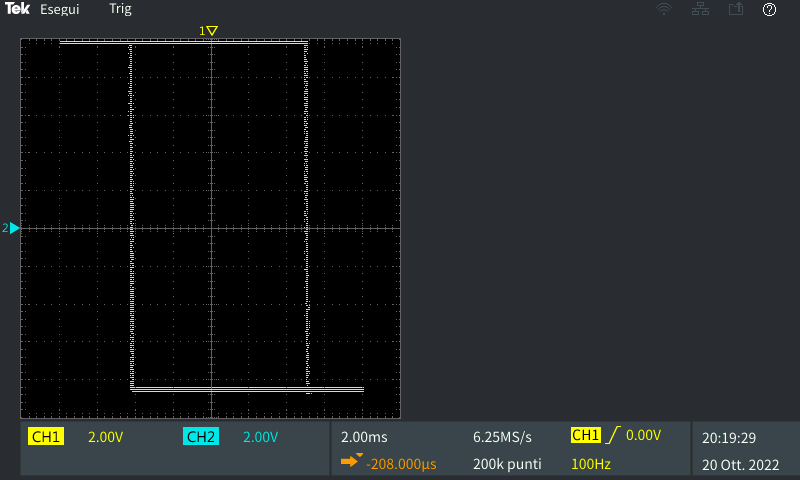
\includegraphics[height=6cm]{immagini/TEK00019}
	\caption{Rappresentazione XY della risposta del circuito con $\mathrm{f= \SI{100}{\hertz}}$.}
	\label{figura:uscita22}
\end{figure}
\todo{Quando f aumenta $->$ visibile slew rate OPAMP $=>$ isteresi non più rettangolare ma a parallelogramma (aggiungere immagini oscilloscopio + spiegazione)}

\newpage\null\newpage % da togliere poi ultimi due comandi
\section{Circuito 3: oscillatore con duty cicle pari a 50\%}
\subsection{Schema del circuito e Funzione di Trasferimento}
Il trigger di Schmitt può essere utilizzato per realizzare un oscillatore. Un oscillatore è un circuito  che produce in uscita una forma d'onda ad una determinata frequenza, entrambi i parametri (forma e frequenza) dipendono sia dai componenti presenti nell'oscillatore che dalle tensioni di alimentazione. \`E un circuito particolare perché è \textit{autoalimentato}, questo significa che non dovremo applicare un segnale in ingresso per osservare il segnale d'uscita (per innescare la reazione è sufficiente un disturbo, ad esempio il rumore dei componenti elettronici).
\begin{figure}[h!]
	\centering
	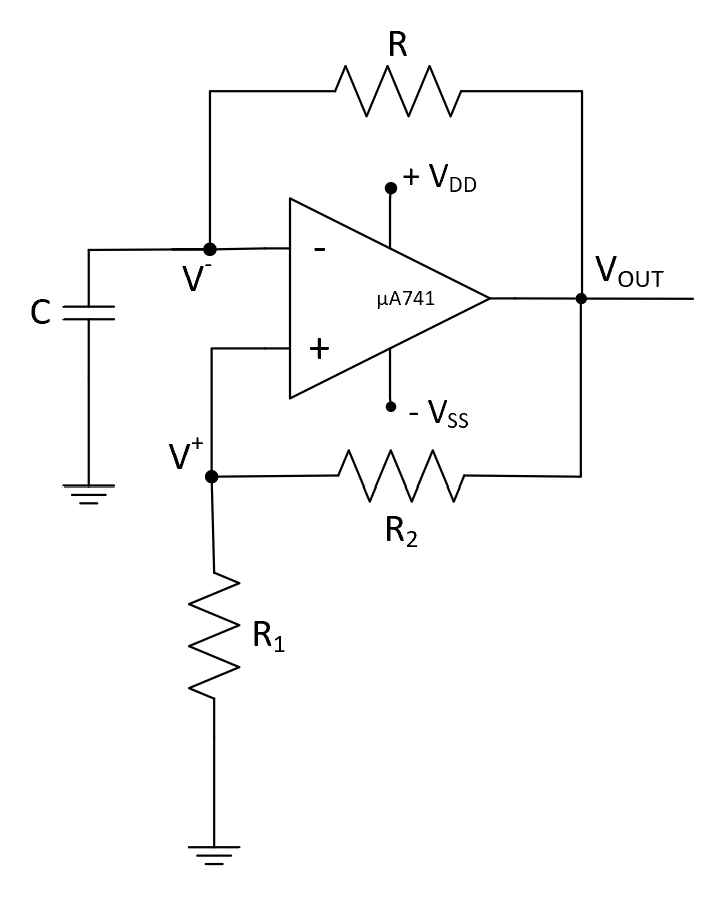
\includegraphics[height=8cm]{immagini/schema3}
	\caption{Schema dell'oscillatore con duty cicle di 50\%.}
	\label{figura:schema3}
\end{figure}
\\Il circuito che realizzeremo produrrà in uscita un'onda quadra. Inizialmente utilizzeremo lo stesso valore per le resistenze $\mathrm{R_1}$ e $\mathrm{R_2}$, quindi le soglie che determinano le transizioni da alto a basso e viceversa sono:
\begin{table}[h!]
	\centering
	\begin{tabular}{cc}
		$\displaystyle{V_H^+=\frac{R_1}{R_1+R_2}\cdot V_{DD}=+\SI{5}{\volt}}$\;\;\;\;\;\;\;\;\;\;\;\;\;\;\;\;\;\;\;\; & $\displaystyle{V_L^+=\frac{R_1}{R_1+R_2}\cdot V_{SS}=-\SI{5}{\volt}}$\\ 
	\end{tabular}
\end{table}
\\Il suo funzionamento sfrutta il processo di carica e scarica di un condensatore su una resistenza. Ipotizziamo che inizialmente il condensatore sia scarico, se $\mathrm{V^-}$ è minore di $\mathrm{V^+}$, l'uscita satura alla tensione positiva e il condensatore si carica attraverso la resistenza $\mathrm{R}$. La tensione ai suoi capi cresce con andamento esponenziale, con costante di tempo $\displaystyle{\tau=R\cdot C}$. Se non ci fosse la soglia $\mathrm{V_H^+}$, la tensione ai capi del condensatore continuerebbe a crescere fino a raggiungere la tensione di saturazione positiva. In questo oscillatore invece, quando la tensione ai capi della capacità raggiunge la soglia $\mathrm{V_H^+}$, si ha che $\mathrm{V^-}$ è maggiore di $\mathrm{V^+}$, di conseguenza l'uscita satura alla tensione negativa. Questo provoca la scarica della capacità sulla resistenza, l'andamento è sempre esponenziale con la stessa costante di tempo $\tau$. Il processo di scarica continua fin quando la tensione ai capi della capacità risulta pari alla soglia inferiore, in questo caso risulta soddisfatta la condizione $V^+>V^-$, e il condesatore ripete il processo di carica. Il comportamento del circuito può essere riassunto così:
\begin{equation}
   \begin{cases}
   [metti formule]
   \end{cases}
\end{equation}
Il periodo di oscillazione dipende dai tempi t1 e t2 [...]
\subsection{Analisi e dati sperimentali}
Utilizzaimo ancora le tre r da 12 k misurate in tabella \ref{table:mis_res1}. Posizioniamo componenti su bb, come mostrato in figura \ref{figura:circuito3} e colleghiamo oscilloscopio, metti fig. ci dà frequenaz di ...
\begin{figure}[h]
	\centering
	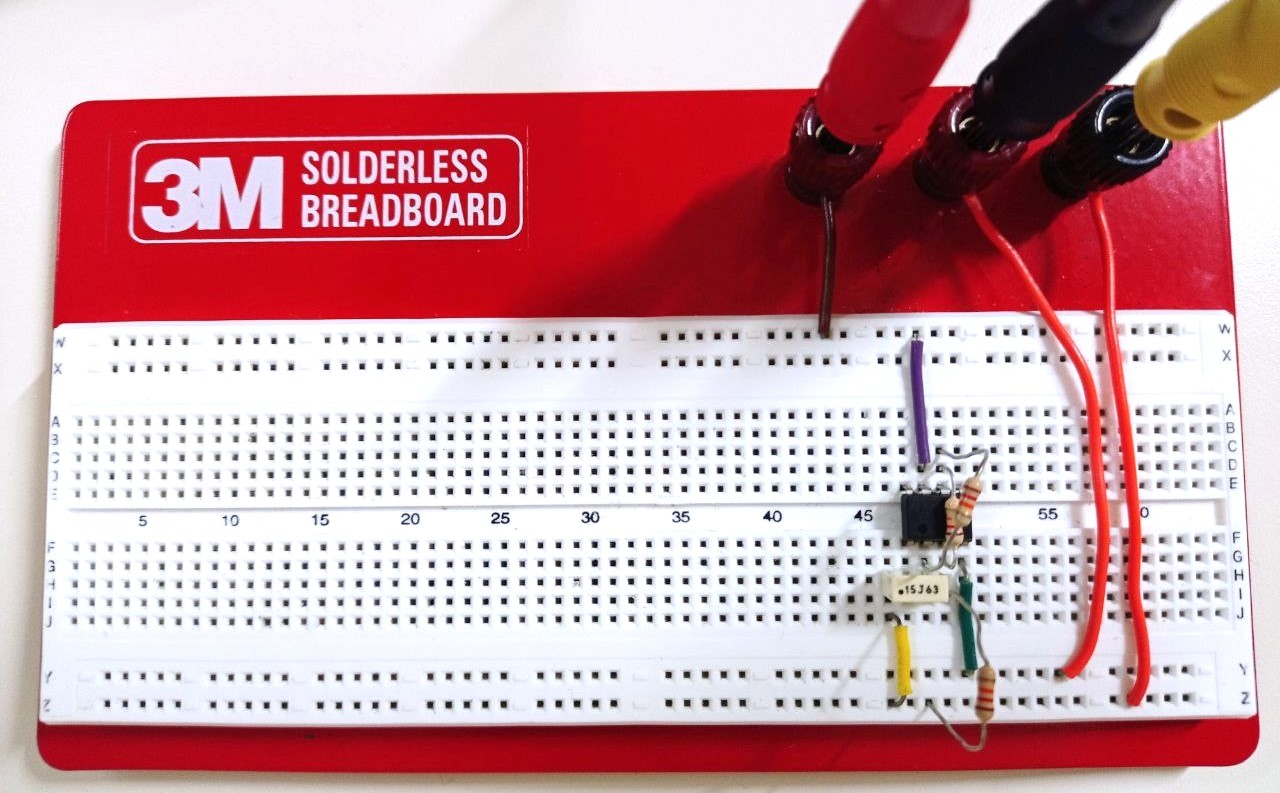
\includegraphics[height=6.2cm]{immagini/circuito3}
	\caption{Fotografia dell'oscillatore con duty cicle pari a 50\% realizzato in laboratorio.}
	\label{figura:circuito3}
\end{figure}
\\Utilizziamo formule per vedere se periodo corretto.
[...]
\\calcolo dc
\\spostamento alimentaziooni e nuove misure
\newpage
\section{Circuito 4: oscillatore con duty cicle diverso da 50\%}
\subsection{Schema del circuito e Funzione di Trasferimento}
spostare alim non buono, quindi con diodi e due r di valore diverso, cerchiamo di realizzare un oscillo con dc != da 50
\begin{figure}[h]
	\centering
	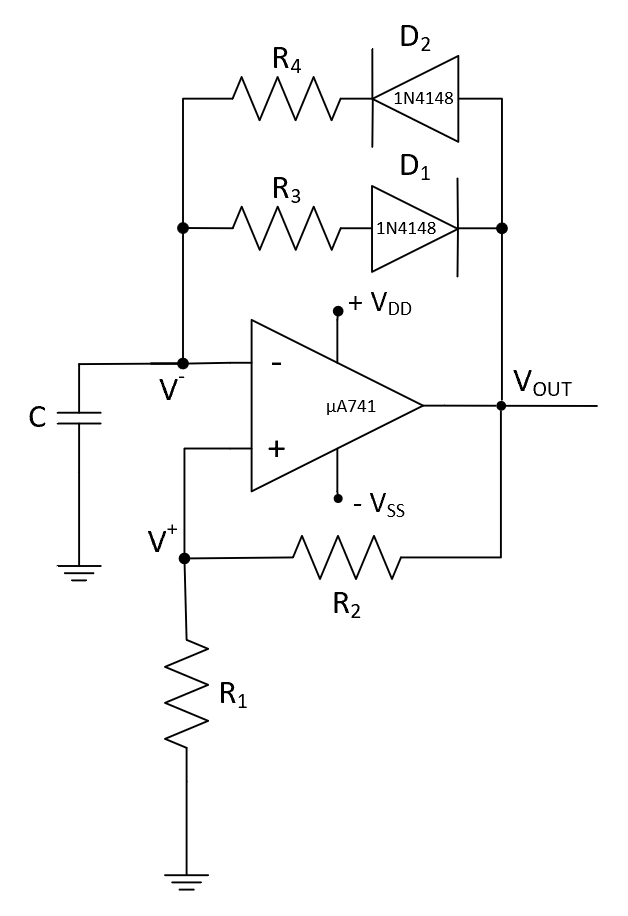
\includegraphics[height=6.2cm]{immagini/schema4}
	\caption{Schema dell'oscillatore con duty cicle diverso da 50\%.}
	\label{figura:schema4}
\end{figure}
\\dc puo essere min magg del 50, rip da valore di r 3 e 4 (metti relazione)
%\noindent La funzione di trasferimento di questo raddrizzatore è:
%\begin{equation}
%   \begin{cases}
	%   \end{cases}
%\end{equation}
\subsection{Analisi e dati sperimentali}
info su bb
\begin{figure}[h!]
	\centering
	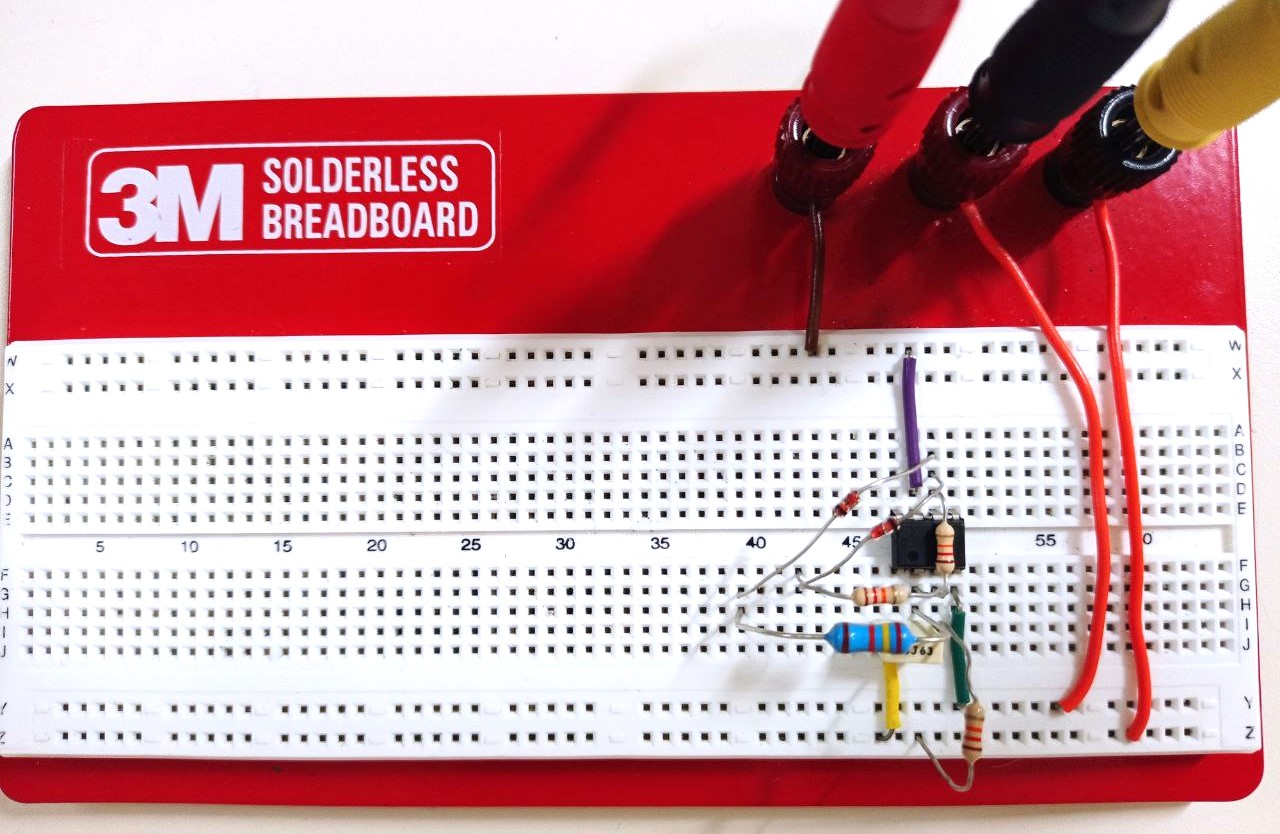
\includegraphics[height=6.2cm]{immagini/circuito4_1.jpg}
	\caption{Fotografia dell'oscillatore con duty cicle maggiore del 50\% realizzato in laboratorio.}
	\label{figura:circuito4_1}
\end{figure}
\\oscillo+analisi misure e formule
\\ora scambiamo verso diodi, cosi da avere r invertite e ripetiasmo analisi. secondo cto in fig \ref{figura:circuito4_2}.
\begin{figure}[h!]
	\centering
	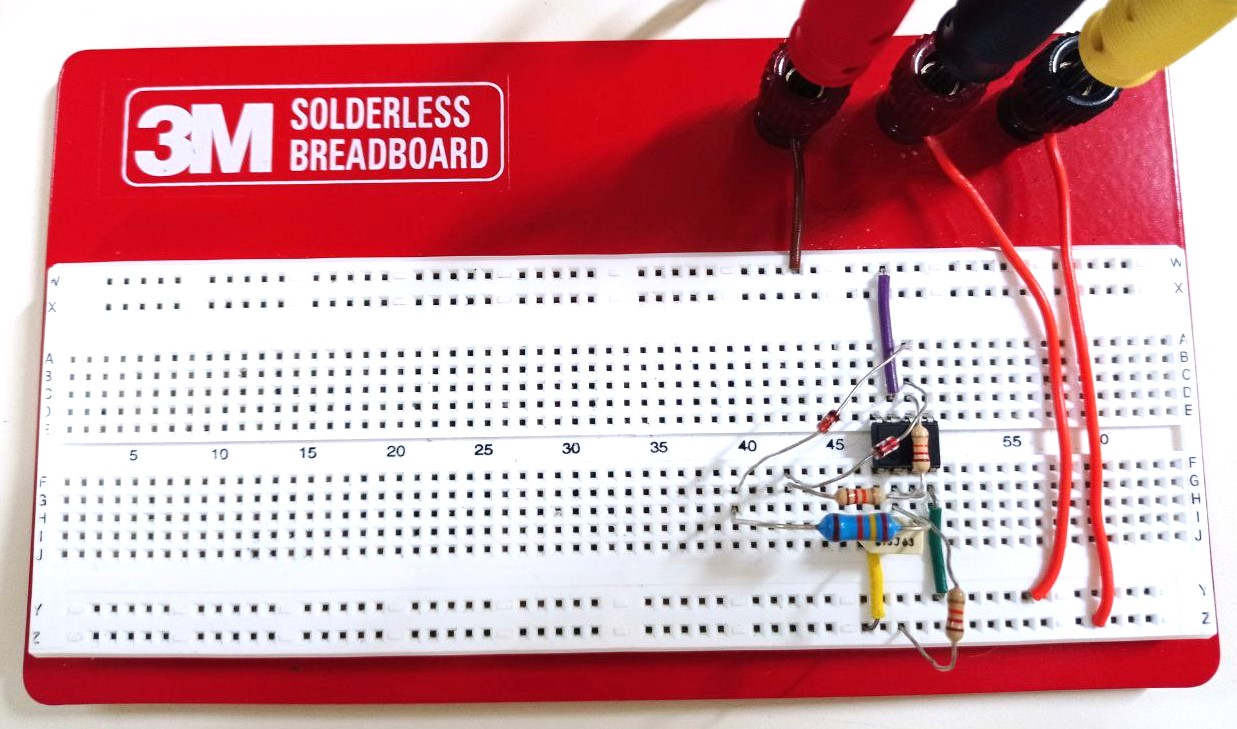
\includegraphics[height=6.2cm]{immagini/circuito4_2.jpg}
	\caption{Fotografia dell'oscillatore con duty cicle minore del 50\% realizzato in laboratorio.}
	\label{figura:circuito4_2}
\end{figure}
\\oscillo+misure

%----------------------------------------------------------------------------------------

\end{document}
